\documentclass{article}
\usepackage[utf8]{inputenc}
\usepackage{hyperref}

\usepackage{graphicx}
\graphicspath{ {./images/} }
\usepackage{wrapfig}

\usepackage[backend=biber,
bibencoding=ascii,
style=mla,
citestyle=numeric,
sorting=ynt
]{biblatex}
\addbibresource{bibliography.bib}


\title{Collaborative Learning: \\
\normalsize Strategies and Platform Development
}
\author{Paul Baier}
\date{April 20, 2020}

\begin{document}

\maketitle

\begin{abstract}
Throughout the past few years there has been a growing interest among educators to use tools to enhance the student learning experience, sometimes referred to as "Learning Objects" (LO) or "Information and Communication Technology (ICT). As a result, more recent research has been directed to the creation of student-centered educational platforms. The goal of this project is to design and develop a highly extensible, open source, game-based webapp. The platform can be used by instructors to create custom and programmable assessment activities and researchers to explore the effects of different hypotheses involving student collaboration in a classroom setting. Depending on an interplay of factors such as class size, the nature of the material, and personal preferences, instructors may have different ideas and notions of what the ideal student collaboration activity should be. In order to cater to the different instructors’ needs, this system gives instructors the ability to control the flow of information between students for a given activity, and allows instructors to define the structure and rules of how a particular activity should be undertaken.
\end{abstract}

\section{Introduction}
A student response system (SRS) is one used in classrooms to get student feedback. There are many SRS games, which we refer to as student response games (SRG).

\section{Literature Review}
In order to identify prior work in the area of educational games we looked at roughly 2000 proceedings from the Frontiers in Education (FIE) conference from 2015-2019. We started our search with the word "kahoot" because our platform's functional design is based off of Kahoot. Within the search results we identified other platforms mentioned that were similar to Kahoot (and therefore also similar to our platform) and recursively searched for those other platforms as well within the proceedings. This search method allowed us to determine other popular platforms researchers were testing that are comparable to Kahoot as well as other SRS/SRG platforms in development. Our search revealed some of the most popular and relevant SRGs currently in production in addition to Kahoot are Socrative\cite{socrative}, Quizizz\cite{quizizz}, and Quizlet\cite{quizlet}. There were also two platforms in development by researchers called Quipid\cite{quipid} and Dysgu\cite{dysgu}.

\subsection{Quizizz}
Of the existing platforms Quizizz most resembles Kahoot and has many customizable features. The main difference between it and Kahoot or our platform is that students move through the quiz at their own pace, limited by the time assigned to each question.

To get started a teacher can either choose a preexisting quiz from a library of quizzes organized by topic or they can create their own. If they choose a pre-made quiz, they can use it as is or copy and edit it to their liking. If they choose to create a new quiz, they can search through existing quizzes for questions in addition to creating their own.

Question types include multiple choice, checkbox (select all the correct answers), fill-in-the-blank, polls, and open-ended (the last two are ungraded but marked as correct in reports). For each question the teacher can specify the amount of time the student has to answer. Scores for answering a question correctly are determined in part by the time it took the student to answer relative to the time length of the question. However, the timer can be disabled in which case the time factor would not be considered when scoring a question.

Once the quiz is made there are three game modes: team, classic, and test. We will only look at team and classic modes as test mode is beyond the scope of our work.

Team mode, as the name suggests, organizes students into teams. In classic mode each student competes by themselves. The main difference between the two modes is that the number of teams needs to be specified by the teacher in team mode and the team scores are based on the cumulative results of the team members. Both team and classic mode share similar gameplay settings. A teacher is able to toggle the timer on or off for the game, shuffle the questions, shuffle the answer options, and allow for a "redemption question" where students are able to retry missed questions. There are also memes that show up between questions that the teacher can toggle off for the game or the student can toggle off for their own experience. Another option teachers have is to either show the correct answer to the student in the game after they answer, show only if the got the question right or wrong, or do not visually indicate a correct or incorrect answer (there is a noise that indicates correct or incorrect regardless of this setting).

Lastly Quizizz has a feature called "Power-ups" which "are single-use abilities designed to increase engagement and participation"\cite{quizizz}. Currently there are nine power-ups that are awarded sporadically to players. Once awarded, an icon appears on the student's screen and they can use it any time by clicking on the icon. An example of a power up is 50-50 which eliminates half of the incorrect answers. This entire system is available in both team and classic mode and can be disable before starting the game.

Described above are only some of the features offered on the Quizizz platform but they represent the most relevant when compared with our design.

\subsection{Socrative}
Socrative is a web application focused on student engagement and tracking. It offers a number of features outside of the scope of our application, however one of its activities, called "Space Race", is comparable.
\begin{wrapfigure}{l}{0.5\textwidth}
    \centering
    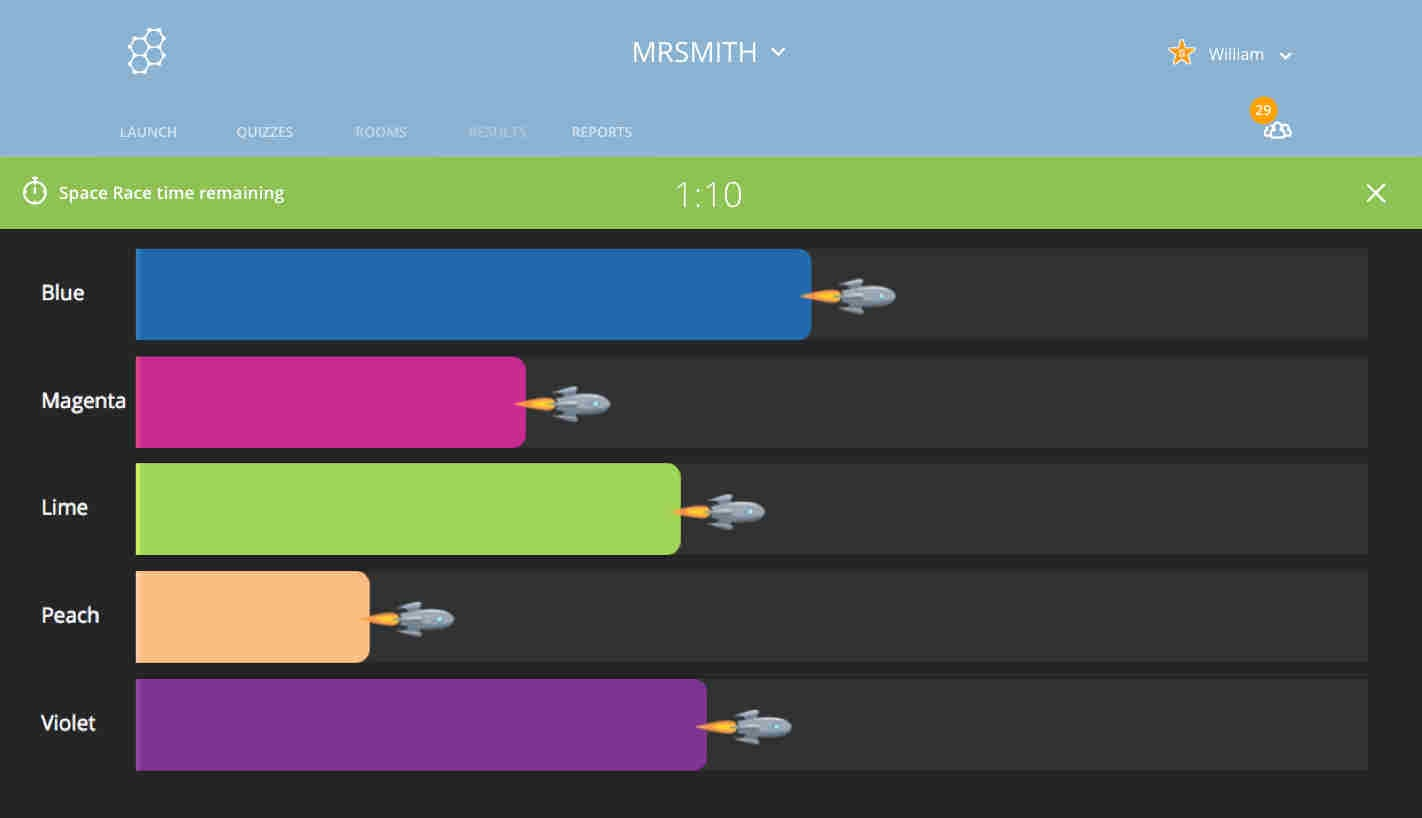
\includegraphics[width=0.5\textwidth]{images/socrative-space_race.jpg}
    \caption{Socrative Space Race \cite{socrative}}
    \label{fig:socrative-space-race}
\end{wrapfigure}
Space Race is a quiz-like game where students are asked a series of questions prearranged by the teacher. Their progress is tracked by little rocket ships (or other icons) that move across the teacher's dashboard when a question is answered correctly (figure \ref{fig:socrative-space-race}). The goal is to be the first individual or team to have their rocket reach across the screen.

Quizzes can be made of multiple choice, true/false, and short answer questions. Other quiz options include the number of teams, how the players are assigned to teams (auto-assigned or student's choice), if the quiz is timed, shuffle the questions, shuffle the answers, show question feedback, show the final score, and if questions can only be attempted once.

\subsection{Quizlet}
Like Socrative, Quizlet is a web application that offers many features to its users. It provides students and teachers with the tools to create interactive study materials based on "sets", which are essentially digital flashcards.
\begin{wrapfigure}{r}{0.5\textwidth}
    \centering
    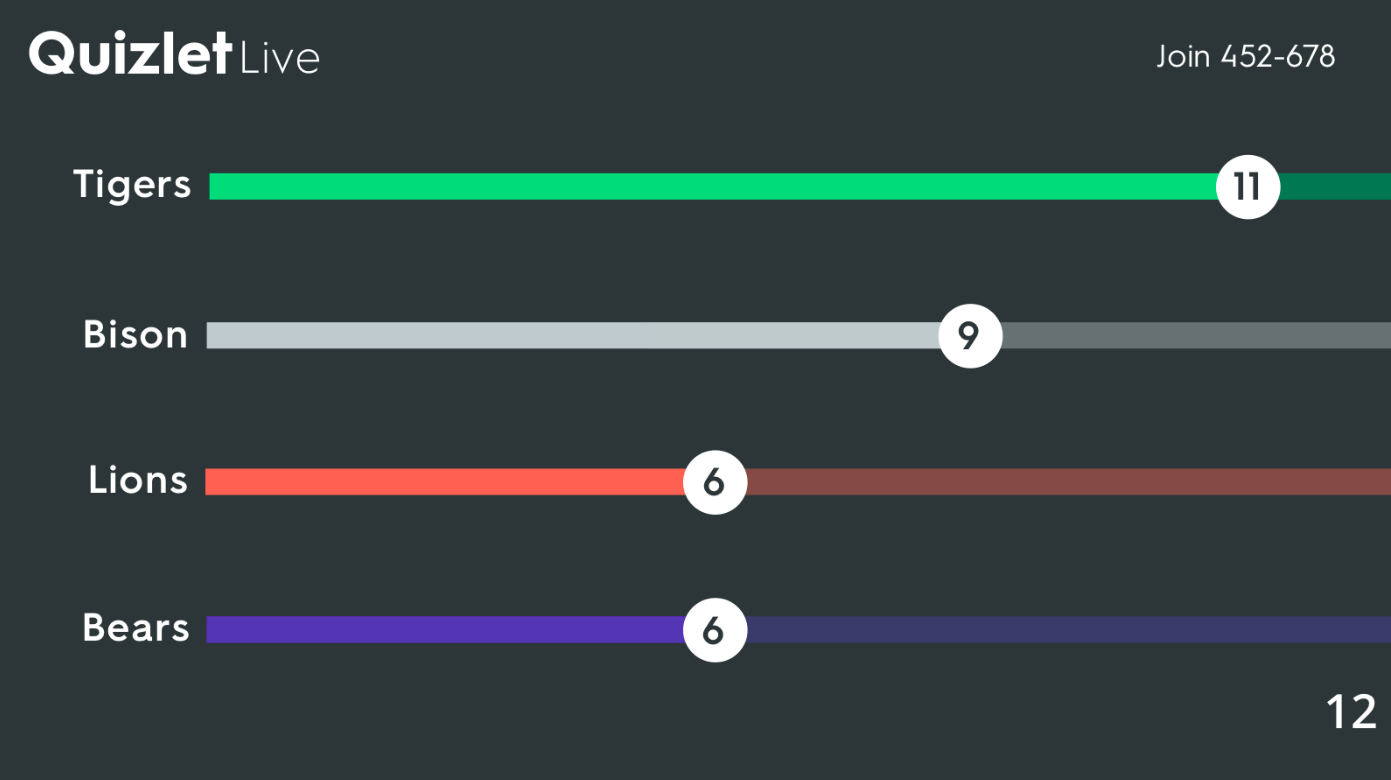
\includegraphics[width=0.5\textwidth]{images/quizlet-live.png}
    \caption{Quizlet Live Dashboard \cite{quizlet}}
    \label{fig:quizlet-live}
\end{wrapfigure}
Each set is made up of any number of "cards" which contain a term "side" and a definition "side". Teachers and students can input the term and definition for their cards and create their own sets.

While most of the features offered by Quizlet do not overlap with our platform there is one, called "Quizlet Live", that is similar.

Quizlet live is a game that asks students multiple choice questions and tracks their progress on the teacher's dashboard (figure \ref{fig:quizlet-live}). The teacher selects the set they want to use for the game and is able to choose between individual and team mode. Once selected the teacher is given the option for the questions to be generated based on the term side of the card or the definition side. The game ends for everyone when the first individual or team answers all of the questions correctly. If a question is answered incorrectly the correct answer is shown and the individual or team starts back at the beginning. Questions are randomly displayed to each player/team. In individual mode there are always four answer options shown in a random order, three of which are answers for other questions in the set.

\begin{wrapfigure}{l}{0.25\textwidth}
    \centering
    
\includegraphics[width=0.25\textwidth]{images/quizlet-team.png}
    \caption{Quizlet Team View \cite{quizlet}}
    \label{fig:quizlet-team}
\end{wrapfigure}

In team mode the number of teams is automatically generated based on the number of players. Students are assigned to a team randomly and the teams can be shuffled by the teacher before the game starts. In the game, the answers to each question are split equally between each member of the team and always displayed on the screen. There are no wrong answers displayed in team mode. For example, if there were 10 questions and two people on one team, then each person on that team would see five answers on their screen. Each answer is the answer to one of the questions but because the answers are divided across all team members, a player will not always have the answer to a question on their screen. It is up to the player with the correct answer to answer the question. Once the question is answered correctly a check mark appears where that answer used to be and the next question is displayed (figure \ref{fig:quizlet-live}).

\subsection{Quipid}
\subsection{Dysgu}



Lorem ipsum dolor sit amet, consectetur adipiscing elit, sed do eiusmod tempor incididunt ut labore et dolore magna aliqua. Ut enim ad minim veniam, quis nostrud exercitation ullamco laboris nisi ut aliquip ex ea commodo consequat. Duis aute irure dolor in reprehenderit in voluptate velit esse cillum dolore eu fugiat nulla pariatur. Excepteur sint occaecat cupidatat non proident, sunt in culpa qui officia deserunt mollit anim id est laborum.

Lorem ipsum dolor sit amet, consectetur adipiscing elit, sed do eiusmod tempor incididunt ut labore et dolore magna aliqua. Ut enim ad minim veniam, quis nostrud exercitation ullamco laboris nisi ut aliquip ex ea commodo consequat. Duis aute irure dolor in reprehenderit in voluptate velit esse cillum dolore eu fugiat nulla pariatur. Excepteur sint occaecat cupidatat non proident, sunt in culpa qui officia deserunt mollit anim id est laborum.

\section{Design}
	\subsection{Languages}
		\subsubsection{Python}
		\subsubsection{Django}
\section{Development}
\section{Features}
\section{Future Work}

\printbibliography[title={Bibliography}]


\end{document}

